\section{Introduction} \label{sec:intro}

%\begin{itemize}
%\item Importance of BX, BX is a solution of view update problem in database.
%\item goodness of
%\item Explanation of put-based BX: BiGUL.
%\item Current status of BiGUL: Fastest BX language in the world
%\item But there is a problem: Efficiency of compose evaluation. The current implementation of BiGUL does not save the intermediate states, the number of get is quadratic. This is not good.
%\item To solve this problem we use an idea: introduce pg : combination of put and get. Then, no information will be lost in a specific condition.
%  an idea from reversible computation: not to lose any information.
%\item We extend pg with several ideas to produce faster implementation.
%\item
%\end{itemize}

%\begin{itemize}
%\item Importance of BX, BX is a solution of view update problem in database.
%\item goodness of
%\item Explanation of put-based BX: BiGUL.
%\item Current status of BiGUL: Fastest BX language in the world
%\item But there is a problem: Efficiency of compose evaluation. The current implementation of BiGUL does not save the intermediate states, the number of get is quadratic. This is not good.
%\item To solve this problem we use an idea: introduce pg : combination of put and get. Then, no information will be lost in a specific condition.
%  an idea from reversible computation: not to lose any information.
%\item We extend pg with several ideas to produce faster implementation.
%\item
%\end{itemize}

%In software, there are strong demands for synchronizing data. In database community this is known as ``the view update problem'' and researched for a long time.
% A Survey to View Update Problem
%As a solution for this problem, bidirectional transformation (BX) is introduced.
The synchronization of data is a common problem. In the database community this problem is known as ``the view update problem'' and has been investigated for a long time~\cite{Bancilhon:1981:USR:319628.319634}. Bidirectional transformation (BX) provides a systematic approach to solving this problem.
Consider a small BX program of $phead$\footnote{The actual program is shown in the next section.}, which consists of two functions: $get$ (for getting the head of an input list) and $put$ (for reflecting the output to the head of the input). Figure \ref{fig:eval-phead} shows an example of the bidirectional behavior of $phead$.
Let $[1,2]$ be the original source~$s$.
The function $get$ is a projection: $get$ of $phead$ picks the first element of the given original source $[1,2]$ and returns $1$ as a view $v$.
%\texttt{get pHead [1,2] = 1}.
%After the view \texttt{v} is obtained, the user can modify the view.
%In this case, the user
%modified the view
%from $1$ to $100$.
%From this updated view, how can the source be updated?
%This is ``the view update problem.''
%To solve this problem, BX provides $put$, an update function on the original source.
%In this example,
Supposing that the view is updated to $100$,
$put$ of $phead$ will construct a new source $s'$ of ${[100,2]}$ from the updated view $v'$ of $100$ and the original source $s$ of $[1,2]$.
%Note that the update to \texttt{s'} uses \texttt{s} and \texttt{v'} as input.
%\texttt{put pHead [1,2] 8 = [8,2]}

\begin{figure}[!t]
  \begin{minipage}{0.3\textwidth}
    \centering
    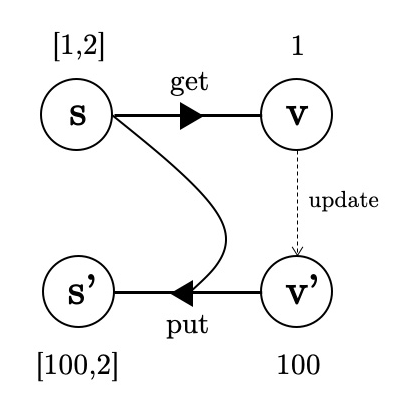
\includegraphics[height=3.5cm]{./fig/fig1.eps}
    \caption{Evaluating $phead$}
    \label{fig:eval-phead}
  \end{minipage}\hfill
  \begin{minipage}{0.7\textwidth}
    \centering
    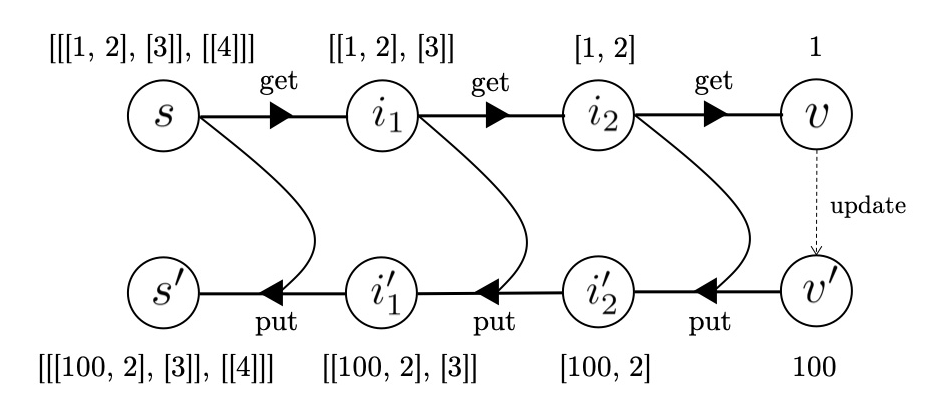
\includegraphics[height=3.5cm]{./fig/fig2.eps}
    \caption{Evaluating $phead \circ phead \circ phead$}
    \label{fig:eval-comp-phead}
  \end{minipage}
\end{figure}
%\vspace*{-5.5mm}


The composition of BX programs is a fundamental construct to build more complex BX programs \cite{Bohannon06relationallenses:, Bohannon:2008:BRL:1328438.1328487}. Let $bx_1$ (defined by $get_{bx_1}$ and $put_{bx_1}$) and $bx_2$ (defined by $get_{bx_2}$ and $put_{bx_2}$) be two bidirectional programs, then their composition $bx_1 \circ bx_2$ is defined by

\minusvspace
\begin{align}
get_{bx_1 \circ bx_2}~s &= get_{bx_2} (get_{bx_1}~s)\\
put_{bx_1 \circ bx_2}~s~v' &= put_{bx_1} s~(put_{bx_2}~ (get_{bx_1}~s)~v')
\end{align}
\minusvspace

\noindent
\textcolor{red}{Note that the order of composition is different from that of the common function composition. We use this order, because it is helpful to understand the behavior if we consider data goes from left to right.}
One feature of this composition is that $put_{bx_1 \circ bx_2}$ needs to call $get_{bx_1}$ to compute the intermediate result for $put_{bx_2}$ to use, which would introduce an efficiency problem if we compute $put$ for composition of many bidirectional programs. Generally, for a composition of $O(n)$ bidirectional programs, we need to call $get$ for $O(n^2)$ times. To be concrete, consider the evaluation of the following composition (which will be used as our running example in this paper):

\minusvspacetwo
\[
lp3 = (phead \circ phead) \circ phead
\]
\minusvspacetwo

\noindent which is illustrated by Figure \ref{fig:eval-comp-phead} with the original source $s$ being ${[[[1,2],[3]],[[4]]]}$ and the updated view ${100}$.
To obtain the final updated source $s'$, $put$ for $lp3$ needs to evaluate $put$ of $phead$ three times. The first is from $i_2$ and $v'$ to obtain $i'_2$, which needs to call $get$ twice to compute $i_2$; the second is from $i_1$ and $i'_2$ to obtain $i'_1$, which needs to call $get$ once, and the last is from $s$ and $i'_1$ to obtain~$s'$, which is just a direct $put$ computation.

%In BX programs, composition of programs is essential for writing various interesting evaluations.
%Because recursions are achieved by compositions, large number of programs include compositions.
%In the BX lens papers \cite{Bohannon06relationallenses:, Bohannon:2008:BRL:1328438.1328487} compositions are also known as central part of BX programs.
%In this section we use a small BX program that contains compositions as a running example, because the programs including recursions can be complicated easily. The running examples are two versions of two composition of $phead$: ($phead \circ phead) \circ phead$ (we call lp3) and $phead \circ (phead \circ phead$) (we call rp3).


%For more various evaluations, we can use the composition of programs. Let us consider another example, a composition of 3 $pHead$s: $pHead \circ pHead \circ pHead$. Figure \ref{fig:eval-comp-phead} illustrates the evaluation of this program where the original source \texttt{s} is \texttt{[[[1,2],[3]],[4]]} and the updated view is \texttt{100}.
%By repetitious evaluation of $get$s of $pHead$, we can obtain the view $v$, \texttt{1}. To obtain the final updated source \texttt{s'}, we need to evaluate $put$ three times. The first put evaluation is from \texttt{i2} and \texttt{v'} and we can obtain \texttt{i2'}.


%By repetitious evaluation of $get$s of $phead$, we can obtain the view $v$, ${1}$. To obtain the final updated source \texttt{s'}, we need to evaluate $put$ three times. The first put evaluation is from \texttt{i$_2$} and \texttt{v'} and we can obtain \texttt{i$_2$'}.

%First, let us see the standard evaluation method of compositions: ``not keeping any intermediate states and obtaining them by evaluation when they are needed.'' In this example, ``intermediate states'' are \texttt{i$_1$} and \texttt{i$_2$}. This method is used in a BX language, BiGUL \cite{Ko:2016:BFV:2847538.2847544,Ko:2017:ABB:3177123.3158129}. The merit of this method is clear semantics and easy to implement. The disadvantage is the number of $get$s will be quadratic when the BX programs' compositions are left associative. In the evaluation of lp3, two $get$s are required for obtaining \texttt{i$_2$} and one $get$ is required for obtaining \texttt{i$_1$}. In total, three $get$s are evaluated. We explain this method in Section~\ref{sect:minbigul}.

One direct solution to avoid this repeated $get$ computation is to compute compositions in a right associative manner. For instance, if we transform $lp3$ to $rp3$:\break

\minusvspacetwo
\vspace{-3mm}
\[
rp3 = phead \circ (phead \circ phead)
\]
\minusvspacetwo
\vspace{-0mm}

\noindent then the $put$ for $rp3$ only needs to compute $get$ of $phead$ twice, one time less than that for $lp3$.
However, this transformation is not always easy to do. For instance, let us consider $breverse$, a bidirectional version of the traditional `reverse' program for reversing a list. It is defined using $\mbox{\it bfoldr}$, a bidirectional version of the traditional $\mbox{\it foldr}$, whose definition  is shown in the last part of Section~\ref{sect:minbigul}. Informally, $\mbox{\it bfoldr}$ is a recursive bidirectional program defined in a way like

\vspace{1mm}
\minusvspacetwo
 \[
 \mbox{\it bfoldr}~bx~\cdots = \cdots  (\mbox{\it bfoldr}~\cdots) \circ bx \cdots
 \]
 \minusvspacetwo

\noindent where the composition is inherently left associative, and the number of composition is dynamically determined by the length of the source list. This makes it hard to do the above transformation statically. The same efficiency problem occurs in all BX languages.


%A part of the definition of $\mbox{\it bfoldr}$, we have $(\product{Replace}{(\mbox{\it bfoldr} \ bx)}) \circ bx$. In this program, recursion occurs on the left-hand side of composition. Because of priority, it is impossible to transform this program to right associative compositions. At the same time, we can not apply program fusion \cite{Wadler:1988:DTP:80099.80104} to this program because actual program is dynamically produced by recursions depending on the length of the input list. Therefore, it is important to have a fast evaluation method for left associative compositions.

\begin{figure}[!t]
  \centering
  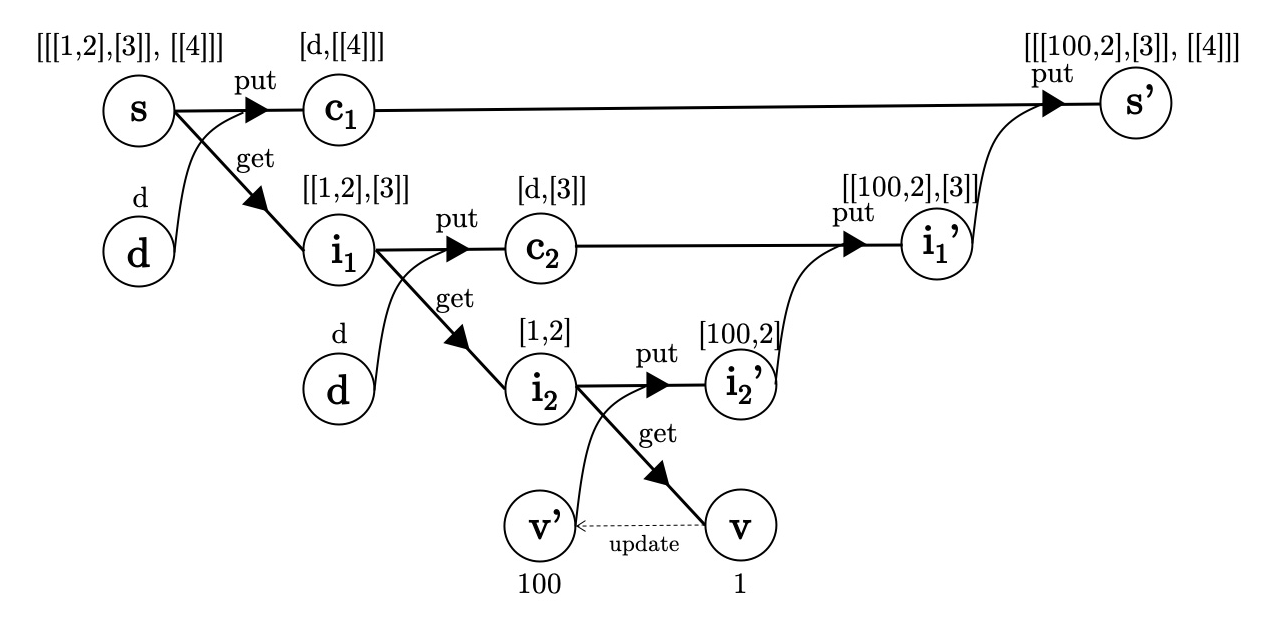
\includegraphics[height=5cm]{./fig/fig3.eps}
  \vspace{-0.25cm}
  \caption{Evaluating $phead \ \circ \ phead \ \circ \ phead$ by keeping complements}
  \vspace{-0.5cm}
  \label{fig:eval-comp-phead-2}
\end{figure}


In this paper, we make the first attempt for seriously considering the efficiency of evaluating BX compositions, and
solve the problem by introducing two methods based on memoization to gain fast evaluation for (left associative) BX compositions.
The first method uses straightforward memoization: ``keeping \emph{intermediate states in a table} and using them when needed''. This avoids repeated $get$ computations and improves the runtime in many cases. However, this simple memoization needs to keep and search values in a table, which may introduce big cost for large inputs. We explain this method in Section~\ref{sect:minbigulm}.

To treat large inputs, we propose the second method based on memoization: ``keeping \emph{complements in a closure} and using them when needed''.
\textcolor{red}{Here, complements are information from sources that makes $get$ injective, which is in turn needed to evaluate $put$.
  In the middle $put$ and $get$ of Figure \ref{fig:eval-comp-phead},
  we use $i_1$, $[[1,2],[3]]$ and $i_2'$, $[100,2]$ to obtain the updated source $[[100,2],[3]]$. However, $[1,2]$ is simply replaced by $[100,2]$ and not used to construct the result. In this case we can use $[..., [3]]$ as a complement.}
The key idea is straightforward: Complements are smaller
% program fragments
than
% the original
intermediate states.
%Therefore this strategy solves the previous two problems.
%Readers might already know that it is a hard problem to obtain complements in general. In our work, thanks to the following finding, it is not hard:
%
%\vspace{2mm}
%In very-well behaved \cite{Foster:2007:CBT:1232420.1232424} BX,% programs,
%$put$ is a complement function for $get$.
%, $get$ can be a complement function for $put$.
%\vspace{2mm}
%
For obtaining complements, we tuple $put$ and $get$, and produce a new function $pg$. Because $put$ produces new complements for $get$, we can shrink the size.
Let us reconsider our example $phead \circ phead \circ phead$ in Figure \ref{fig:eval-comp-phead-2}, where $c_1$ and $c_2$ are complements and $d_1$ and $d_2$ are valid views for $s$ and~$i_1$. Here, two points are worth noting. First, after evaluating the leftmost $pg$, the original source $s$ need not be kept because its complete contents are in $c_1$ and~$i_1$. Second, the complements are smaller than the intermediate states in Figure~\ref{fig:eval-comp-phead}.
%This evaluation looks better than previous two strategies: this does not require repeated evaluation and require smaller storage than the original sources.
Actually, this simple
% combined
$pg$ alone is not yet effective for left associative compositions because it requires two more $put$s, which can be seen on the right side of Figure \ref{fig:eval-comp-phead-2}. To achieve an efficient evaluation, we combine two techniques, lazy update and lazy evaluation. We explain this second method and all optimizations in Section~\ref{sect:xpg}.

Both methods have been fully implemented for \emph{minBiGUL}, a core bidirectional language, which is a subset of the full bidirectional language \emph{BiGUL}. The experimental results show that our methods are much faster than the original evaluation strategy.
We give detailed experimental results in Section~\ref{sect:experiments}, discuss related work in Section~\ref{sect:related}, and conclude in Section~\ref{sect:conclusion}.

Although we will introduce the basics of bidirectional transformation in the next session, it is not complete due to space limitations. Please refer BiGUL papers \cite{Ko:2016:BFV:2847538.2847544, Ko:2017:ABB:3177123.3158129} for the details if needed.

%Due to space limitations, we assume the reader is familiar with the basic concepts of bidirectional transformation.


%The contributions of this paper are the following.

%\begin{itemize}
%\item This is the first attempt for seriously considering efficiency of evaluation of BX compositions. Our methods are better than or similar to the results by the original method in BiGUL for all test cases.
%\item We show that memoization is effective for achieving evaluation efficiency in BX languages.
%\item In BX, as far as authors know optimization by $get$ and $put$ more tight is the first attempt.
%\item Although we focus on a BX language BiGUL in this paper, these techniques can be potentially used in other BX languages.
  % \begin{itemize}
    % Although the first strategy is implemented in BiGUL, the second and third strategies are introduced by this paper.
%  \item Thanks to introduction of the strategies, it is possible to compare the evaluation strategies.
%  \item Improvement of evaluation efficiency
%  \end{itemize}
%\item Approaches used in strategy 3
%  \begin{itemize}
%  \item
% \item Optimization tequniques by tupling, and lazy update
%  \item These tequniques can be potentially used in other BX languages
%  \end{itemize}
%\end{itemize}
